
\begin{center}
\Huge
Funktioner af to variable
\end{center}

\section*{Indledende eksempler}
\stepcounter{section}

Vi betragtede sidst planer og kugler i rummet. På samme måde som at en linje både kan beskrives som en funktion og ved en ligning kan et plan også beskrives som en funktion. 
\begin{exa}
	En funktion $f$ er givet ved
	\begin{align*}
		f(x,y) = ax+by+c.
	\end{align*}
	Denne funktion beskriver en plan i rummet. Dette kan ses ved at sætte $f(x,y)=z$. Så har vi
	\begin{align*}
		f(x,y) = ax+by+c \ &\Leftrightarrow \ z = ax +by + c \\
		&\Leftrightarrow \ ax+by-z+c = 0,
	\end{align*}
	hvilket vi har set er ligningen for en plan. 
\end{exa}
\begin{exa}
	En plan $L$ skærer gennem punktet $(1,2,3)$ og har vektoren $\vv{n}$ givet ved
	\begin{align*}
		\vv{n} = 
		\begin{pmatrix}
			-2 \\ 5 \\ 3
		\end{pmatrix}
	\end{align*}
	som normalvektor. Vi kan bestemme en funktion, der har denne plan som graf. Vi bestemmer først planens ligning.
	\begin{align*}
		-2(x-1)+5(y-2)+3(z-3) = 0\ &\Leftrightarrow \ -2x+2+5y-10+3z-9 = 0 \\
								   &\Leftrightarrow	\  -2x+5y-17=-3z \\
								   &\Leftrightarrow	\ z= f(x,y) = \frac{2}{3}x-\frac{5}{3}y+\frac{17}{3}.
	\end{align*}
	Denne funktion vil altså have $L$ som graf.
\end{exa}

\begin{exa}
	Kuglens ligning har vi set er givet ved
	\begin{align*}
		x^2 + y^2 + z^2 = r^2,
	\end{align*}
	hvor $r$ er kuglens radius og $C(0,0,0)$ er kuglens centrum. Vi kan ikke beskrive kuglens overflade ved et funktionsudtryk af samme grund som vi ikke kan beskrive 
	cirklen ved et funktionsudtryk - vi kan ikke have to funktionsværdier til samme input i funktionen. Vi vælger derfor at beskrive den ovre halvkugle af kuglen, og vi tager 
	udgangspunkt i kuglens ligning. 
	\begin{align*}
		(x)^2 + (y)^2 + (z)^2 = r^2 \ &\Leftrightarrow \ r^2 - x^2 - y^2 = z^2 \\
		\Leftrightarrow  \pm \sqrt{r^2-x^2-y^2} = z.
	\end{align*}
	Vi er interesserede i den øvre halvkugle. Derfor bruger vi den positive løsning. Dette giver os funktionen 
	\begin{align*}
		z=f(x,y) = \sqrt{r^2-x^2-y^2},
	\end{align*}
	hvis graf består af den øvre halvkugle af kuglen med radius $r$ og centrum i origo. Det er desuden et krav, at $r^2 \geq x^2+y^2$.
\end{exa}
\begin{exa}
	En kugle har radius 3 og centrum i $(0,0,0)$. Den øvre halvkugle af denne kugle kan beskrives af funktionen $f$ givet ved
	\begin{align*}
		f(x,y) = \sqrt{9-x^2-y^2}.
	\end{align*}
	Grafen for denne funktion kan ses af Fig. \ref{fig: kugle}.
	\begin{figure}[H]
		\centering
		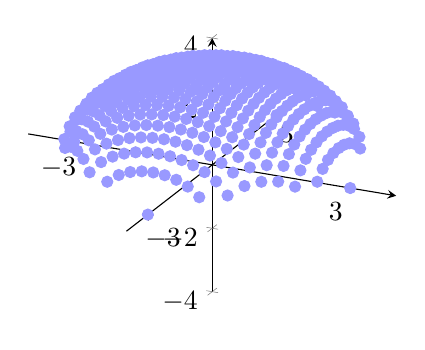
\begin{tikzpicture}
			\begin{axis}[axis lines = middle, 
			xmin = -4, xmax = 4,
			ymin = -4, ymax = 4,
			zmin = -4, zmax = 4
			, xtick = {-3,3}
			, ytick = {-3,3}
			, ztick = {}]
				\addplot3[domain = -3:3, domain y = -3:3,only marks, blue!40] {(9-x^2-y^2)^(0.5)};
			\end{axis}
		\end{tikzpicture}
		\caption{Øvre halvkugle}
		\label{fig:kugle}
	\end{figure}
\end{exa}

\begin{exa}
	En vigtig funktion af to variable er funktionen $f$ givet ved
	\begin{align*}
		f(x,y) = x^2+y^2.
	\end{align*}
	Grafen for denne funktion er en slags tredimentionel parabel - en \textit{paraboloide}. Denne kan ses af Fig. \ref{fig:paraboloide}
		\begin{figure}[H]
		\centering
		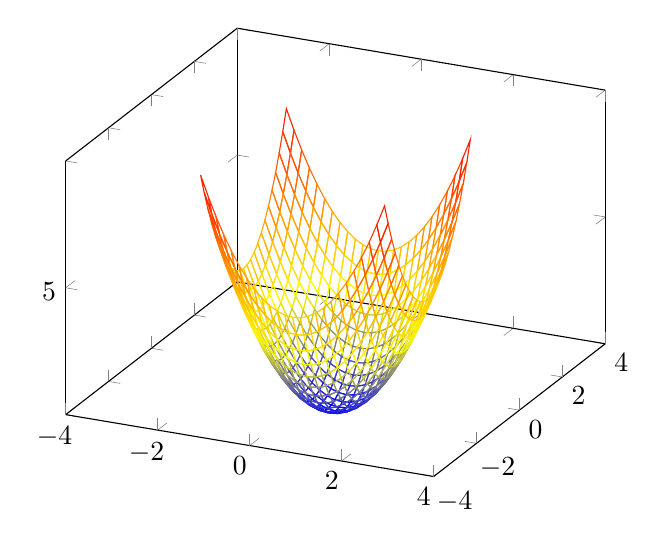
\begin{tikzpicture}
			\begin{axis}[
			xmin = -4, xmax = 4,
			ymin = -4, ymax = 4,
			zmin = --1, zmax = 9]
				\addplot3[domain = -2:2, domain y = -2:2,mesh] {x^2+y^2};
			\end{axis}
		\end{tikzpicture}
		\caption{Paraboloide}
		\label{fig:paraboloide}
	\end{figure}
\end{exa}

\section*{Opgave 1}
En funktion $f$ er givet ved
	\begin{align*}
		f(x,y) = x^2+2y.
	\end{align*}
\begin{enumerate}[label=\roman*)]
	\item Bestem $f(2,4)$, $f(-3,3)$ og $f(3,-3)$.
	\item Bestem to løsninger til ligningen $f(x,y) = 0$. Hvor mange løsninger har den?
\end{enumerate}
\section*{Opgave 2}
En funktion $f$ er givet ved 
\begin{align*}
	f(x,y) = \sqrt{x} + 3y^2.
\end{align*}
\begin{enumerate}[label=\roman*)]
	\item Hvilke af punkterne $(4,1,5)$, $(1,2,3)$ og $(2,1,\sqrt{2}+3)$ ligger på grafen for $f$?
	\item Bestem en løsning til ligningen $f(x,y) = 0$. Kan du bestemme antallet af løsninger til ligningen?
\end{enumerate}
\section*{Opgave 3}
\begin{enumerate}[label=\roman*)]
	\item En plan $L$ går gennem punktet $(-5,4,2)$ og har vektoren $\vv{n}$ givet ved
	\begin{align*}
		\vv{n} = 
		\begin{pmatrix}
			6 \\ 3 \\ -1
		\end{pmatrix}.
	\end{align*}
	Bestem en funktion $f$, der har $L$ som graf. Brug denne funktion til at afgøre, om punktet $(1,1,1)$ ligger på $L$.
	\item En plan $L$ går gennem punktet $(2,4,8)$ og har vektoren $\vv{n}$ givet ved
	\begin{align*}
		\vv{n} = 
		\begin{pmatrix}
			3 \\ -4 \\ -3
		\end{pmatrix}.
	\end{align*}
	Bestem en funktion $f$, der har $L$ som graf. Brug denne funktion til at afgøre, om punktet $(0,1,4)$ ligger på $L$.
\end{enumerate}

\section*{Opgave 4}
\begin{enumerate}[label=\roman*)]
	\item En kugle $K$ med centrum i origo har radius $7$. Bestem en funktion $f$, der har den øvre halvkugle af $K$ som graf for funktionen. Brug denne funktion til at afgøre, 
	om punktet $(0,0,9)$ ligger på kuglen. 
	\item En kugle $K$ med centrum i origo har radius $\sqrt{3}$. Bestem en funktion $f$, der har den nedre halvkugle af $K$ som graf for funktionen. Brug denne funktion til at 
	afgøre, 	om punktet $(-1,1,-\sqrt{3})$ ligger på kuglen. 
\end{enumerate}

\section*{Opgave 5}
\begin{enumerate}[label=\roman*)]
	\item Vis, at den øvre halvkugle for en kugle med centrum i $(x_0,y_0,z_0)$ og radius $r$ kan beskrives ved grafen for funktionen $f$ givet ved
	\begin{align*}
		f(x,y) = \sqrt{r^2-x^2-x_0^2+2xx_0-y^2-y_0^2+2yy_0} +z_0
	\end{align*}
	\item Brug dette til at bestemme en funktion, hvis graf er den øvre halvkugle for en kugle med centrum i $(1,4,3)$ og radius $2$.
\end{enumerate}